\footnotesize
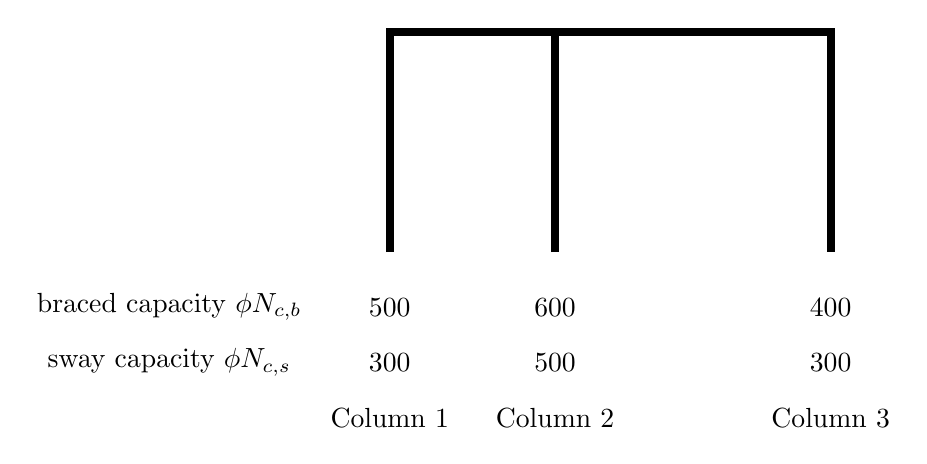
\begin{tikzpicture}[scale=.7]
\begin{scope}
\FixedSupport{0,0}
\FixedSupport{3,0}
\FixedSupport{8,0}
\draw[line width=1mm](0,0)--++(0,4)--++(8,0)--++(0,-4)(3,0)--++(0,4);
\setstructmech{convention=direction}
\node at(-4,-1){braced capacity $\phi{}N_{c,b}$};
\node at(0,-1){\SI{500}{\kn}};
\node at(3,-1){\SI{600}{\kn}};
\node at(8,-1){\SI{400}{\kn}};
\node at(-4,-2){sway capacity $\phi{}N_{c,s}$};
\node at(0,-2){\SI{300}{\kn}};
\node at(3,-2){\SI{500}{\kn}};
\node at(8,-2){\SI{300}{\kn}};
\node at(0,-3){Column 1};
\node at(3,-3){Column 2};
\node at(8,-3){Column 3};
\end{scope}
\end{tikzpicture}